% demo-3min.tex — ThetaSwap 3-Minute Demo Slide Deck
% Shape Rotator 2026 — Encode Club Hackathon Finals

\documentclass[aspectratio=169]{beamer}

% ── Theme and Colors ─────────────────────────────────────────────────────────
\usetheme{Madrid}
\definecolor{thetablue}{RGB}{20,40,80}

\setbeamercolor{structure}{fg=thetablue}
\setbeamercolor{palette primary}{bg=thetablue,fg=white}
\setbeamercolor{palette secondary}{bg=thetablue!80,fg=white}
\setbeamercolor{palette tertiary}{bg=thetablue!60,fg=white}
\setbeamercolor{palette quaternary}{bg=thetablue,fg=white}
\setbeamercolor{frametitle}{bg=thetablue,fg=white}
\setbeamercolor{title}{fg=white,bg=thetablue}
\setbeamercolor{subtitle}{fg=white}
\setbeamercolor{author}{fg=white}
\setbeamercolor{date}{fg=white}
\setbeamercolor{institute}{fg=white}
\setbeamercolor{block title}{bg=thetablue,fg=white}
\setbeamercolor{block body}{bg=thetablue!5,fg=black}
\setbeamercolor{item}{fg=thetablue}
\setbeamercolor{normal text}{fg=black,bg=white}

\setbeamertemplate{navigation symbols}{}
\setbeamertemplate{headline}{}

% ── Packages ─────────────────────────────────────────────────────────────────
\usepackage{amsmath,amssymb}
\usepackage{array}
\usepackage{booktabs}
\usepackage{graphicx}
\usepackage{xcolor}
\usepackage{natbib}
\bibliographystyle{abbrvnat}

% ── Macros ───────────────────────────────────────────────────────────────────
\newcommand{\AT}{A_T}
\newcommand{\ThetaSum}{\Theta}
\newcommand{\PosCount}{N}
\newcommand{\ATnull}{A_T^{1/\PosCount}}
\newcommand{\DeltaPlus}{\Delta^{+}}
\newcommand{\DeltaStar}{\Delta^{*}}
\newcommand{\thetapos}{\theta}
\newcommand{\blocklife}{\ell}

% ── Title Metadata ───────────────────────────────────────────────────────────
\title{ThetaSwap: Adverse Competition Oracle}
\author{ThetaSwap}
\date{Shape Rotator 2026}

% ══════════════════════════════════════════════════════════════════════════════
\begin{document}

% ── Slide 1: Title ───────────────────────────────────────────────────────────
\begin{frame}[plain]
\titlepage
\end{frame}

% ── Slide 2: Thesis ──────────────────────────────────────────────────────────
\begin{frame}{}
\vfill
\begin{center}
\Large
Fee revenue is not equally distributed.\\[6pt]
The competition for it is a risk.
\end{center}

\vfill

\begin{flushright}
\footnotesize\itshape
\citet{macrapis2024permissionless},\;
\citet{capponi2024jit},\;
\citet{aquilina2024dealers},\;
\citet{milionis2024flair}
\end{flushright}
\end{frame}

% ── Slide 3: Aquilina — Fee Concentration Evidence ───────────────────────────
\begin{frame}{Approximately 7\% of LPs capture around 80\% of trading fee revenue}

\begin{center}
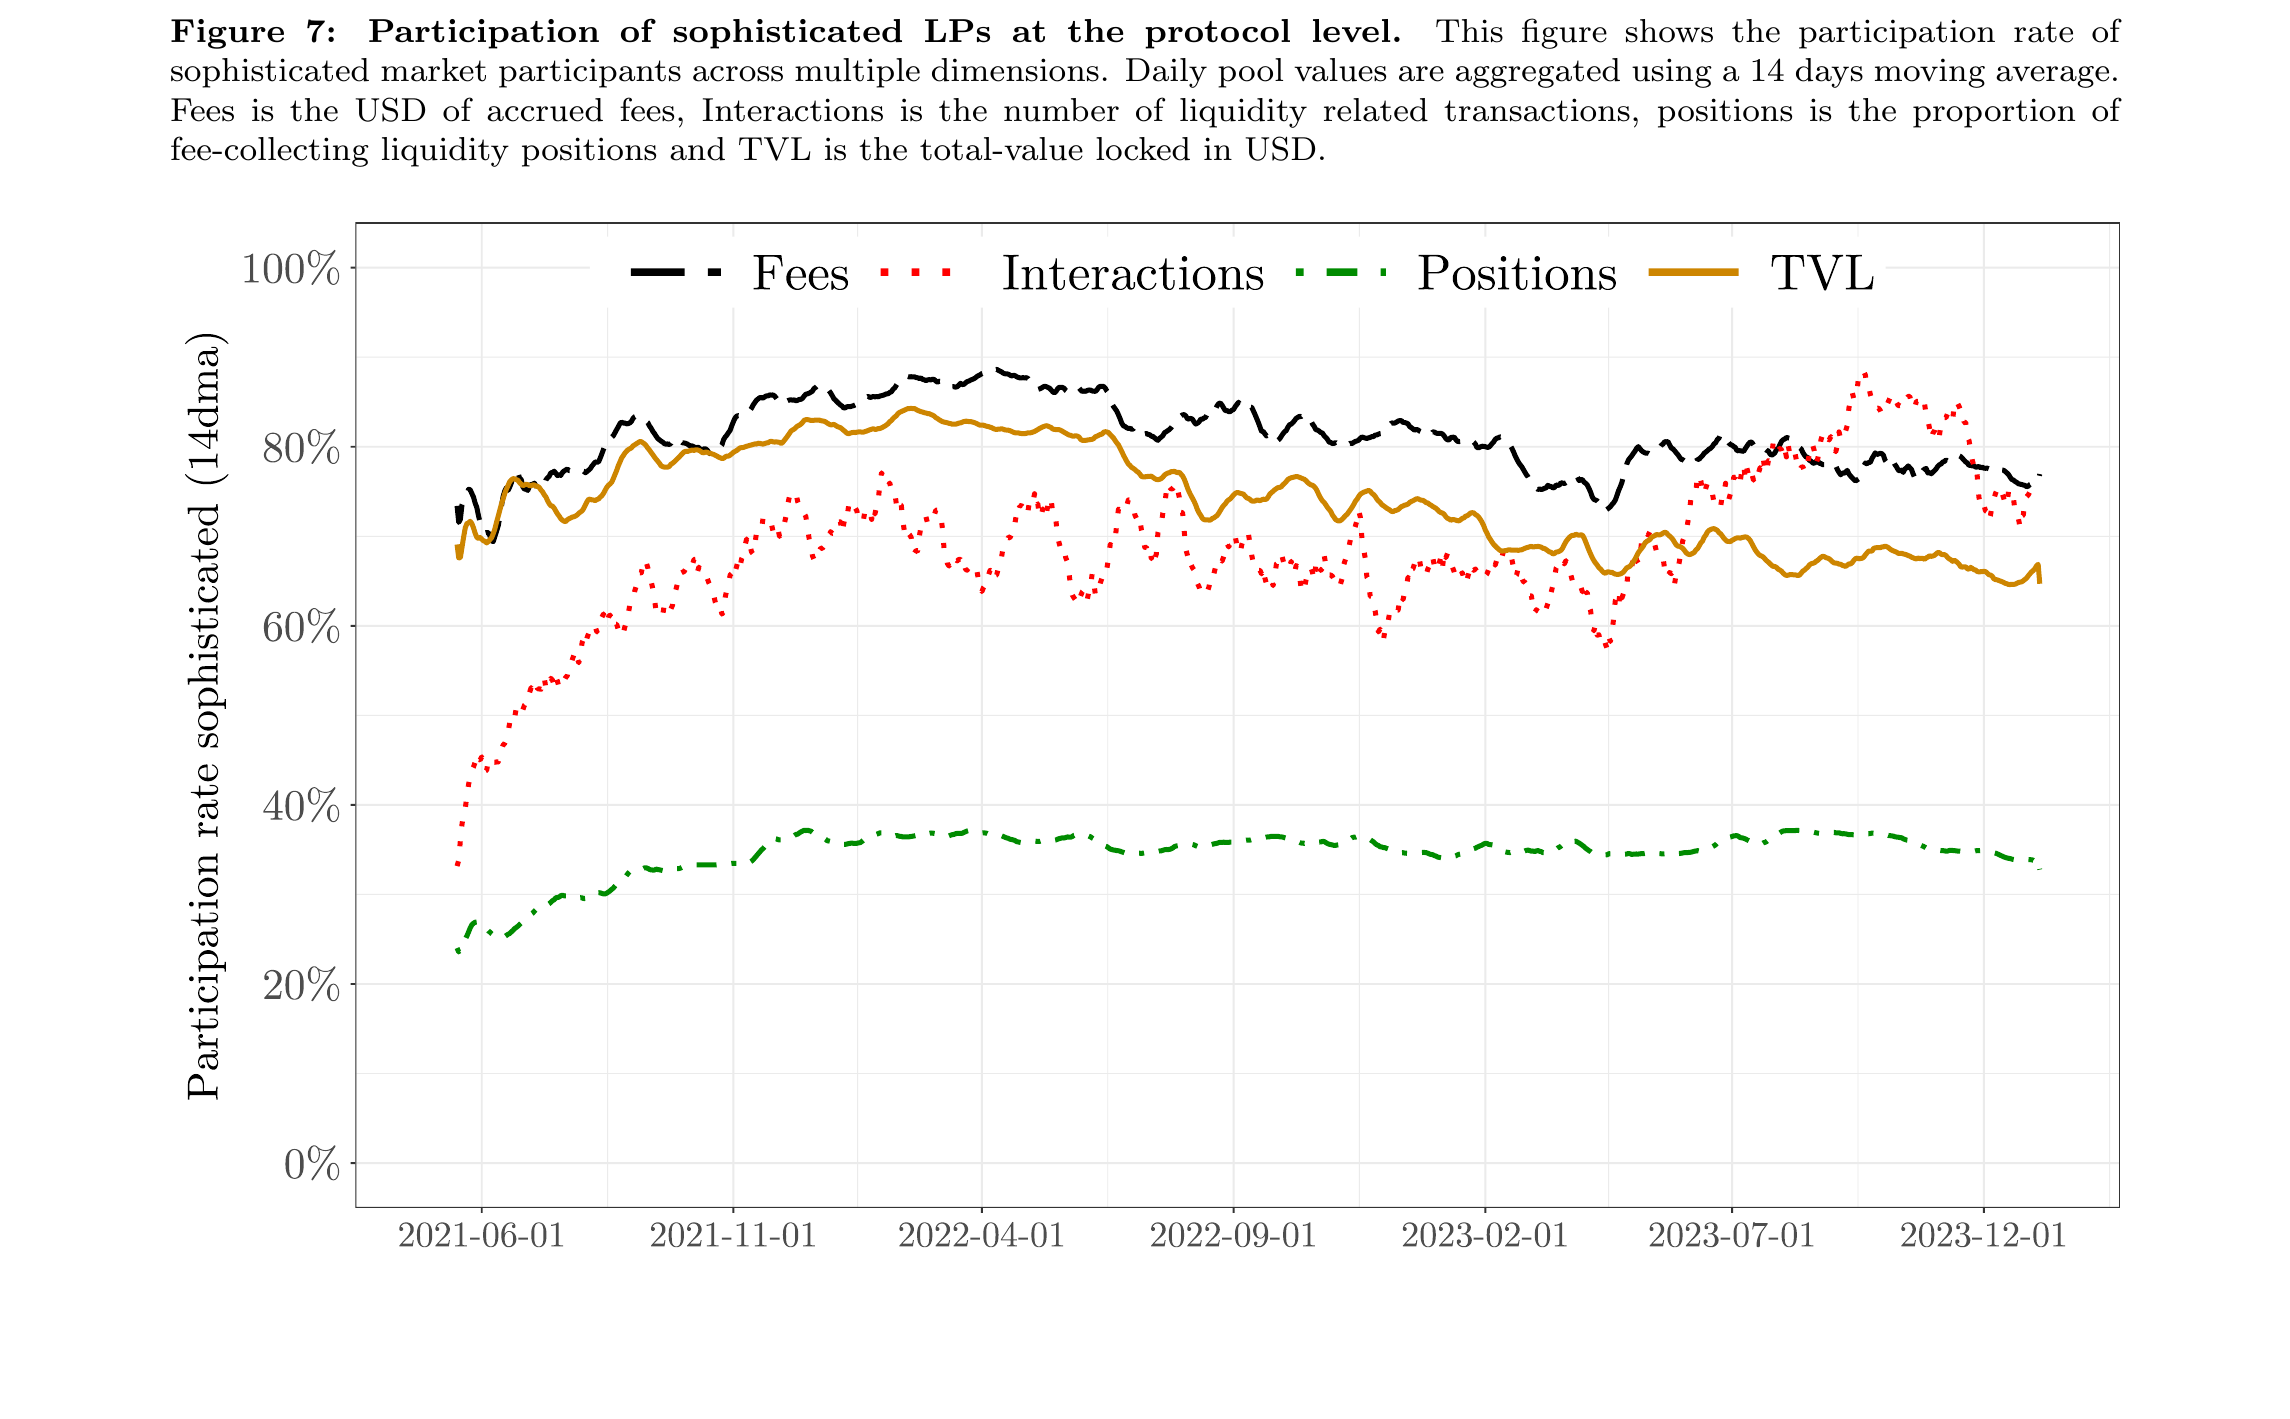
\includegraphics[width=0.80\textwidth,height=0.62\textheight,keepaspectratio]{../figures/aquilina-fig7-participation.png}
\end{center}

\begin{flushright}
\small\itshape
Source: \citet{aquilina2024dealers}, Figure~7
\end{flushright}
\end{frame}

% ── Slide 4: Structural — Competition Harms LPs ─────────────────────────────
\begin{frame}{}
\vfill
\begin{center}
\Large
JIT liquidity creates adverse competition ---\\[6pt]
this is structural, not incidental.
\end{center}

\vfill

\begin{flushright}
\footnotesize\itshape
\citet{capponi2024jit},\;
\citet{macrapis2024permissionless}
\end{flushright}
\end{frame}

% ── Slide 5: Pivot — Can you price it? ───────────────────────────────────────
\begin{frame}{}
\vfill
\begin{center}
\Large
Metrics exist to capture LP competitiveness.\\[12pt]
\textbf{\large But can you price it? Can you hedge it?}
\end{center}

\vfill

\begin{flushright}
\footnotesize\itshape
\citet{milionis2024flair}
\end{flushright}
\end{frame}

% ── Slide 6: The Oracle — FCI Formula ────────────────────────────────────────
\begin{frame}{The Oracle: Fee Concentration Index}

\begin{center}
{\Large $\fbox{$\DeltaPlus = \max\!\bigl(0,\; \AT - \ATnull\bigr)$}$}
\end{center}

\bigskip

\renewcommand{\arraystretch}{1.6}
\begin{tabular}{@{}r@{\;=\;}l@{\quad}p{7cm}@{}}
$\AT$ & $\bigl(\sum_k \thetapos_k \cdot x_k^2\bigr)^{1/2}$
  & fee concentration index \\
$x_k$ & $L_k / \sum_j L_j$
  & liquidity share $\approx$ fee share \\
$\thetapos_k$ & $1/\blocklife_k$
  & turnover --- short-lived positions weigh more \\
$\ATnull$ & $\sqrt{\ThetaSum / \PosCount^2}$
  & competitive null (equal shares) \\
\end{tabular}

\bigskip

\begin{center}
$\DeltaPlus > 0$: fees more concentrated than equilibrium.\\[2pt]
$\DeltaPlus = 0$: fair competition --- no adverse regime.
\end{center}

\end{frame}

% ── Slide 7: Evidence + Backtest — Key Numbers ──────────────────────────────
\begin{frame}{Validation: 600 Real ETH/USDC Positions, 41 Days}

\renewcommand{\arraystretch}{1.5}
\begin{center}
\small
\begin{tabular}{@{}l r@{}}
\toprule
\textbf{Econometric model} & \\
\midrule
Turning point (protective $\to$ adverse) & \textbf{9\% fee dispersion} \\
Marginal exit effect above threshold & \textbf{+2.3 pp} per \% \\
Willingness to pay for protection & \textbf{10\% above hourly fees} \\
\midrule
\textbf{Backtest} (\$200K seed, power-squared payoff) & \\
\midrule
Positions better off hedged & \textbf{18.8\%} \\
Trigger frequency & \textbf{1 day in 41} \\
\bottomrule
\end{tabular}
\end{center}

\medskip

\begin{center}
\textit{Demand exists. It is priceable. The risk profile is textbook insurance.}
\end{center}

\end{frame}

% ── Slide 8: Roadmap ─────────────────────────────────────────────────────────
\begin{frame}{What's Next}

\vfill

\renewcommand{\arraystretch}{2.0}
\begin{tabular}{@{}cl@{}}
\textbf{1.} & Validate across more pools and asset pairs \\
\textbf{2.} & Extend the oracle to other protocols \\
\textbf{3.} & The insurance market --- the CFMM to trade this risk on-chain \\
\end{tabular}

\vfill

\end{frame}

% ── References (hidden, needed for citation resolution) ──────────────────────
\begin{frame}[allowframebreaks]{References}
\footnotesize
\bibliography{../model/references}
\end{frame}

\end{document}
